\chapter{Cap\'{\i}tulo 1: Propiedades de la Membrana de  \textit{Staphyloccocus aureus} y Resistencia de la Bacteria}
\section{La membrana Bacteriana y sus compuestos presentes}\label{ss:mem}
Seg\'{u}n el tipo de membrana que posean las bacterias, est\'{a}s pueden clasificarse en dos grandes clases: las bacterias Gram positivas y las bacterias Gram negativas. Las bacterias Gram positivas poseen una sola bicapa lip\'{i}dica envuelta en una capa compuesta por unos pol\'{i}meros de az\'{u}cares y amino\'{a}cidos llamados peptidoglicando (ver figura \ref{fig:mem}), mientras que las membranas de bacterias Gram negativa poseen dos bicapas lip\'{i}dicas. Ya que \textit{Staphylococcus aureus} es una bacteria Gram positiva se discutir\'{a} principalmente la composici\'{o}n de la membrana de las bacterias Gram Positivas.\\

\begin{figure}[h]
\begin{center}
  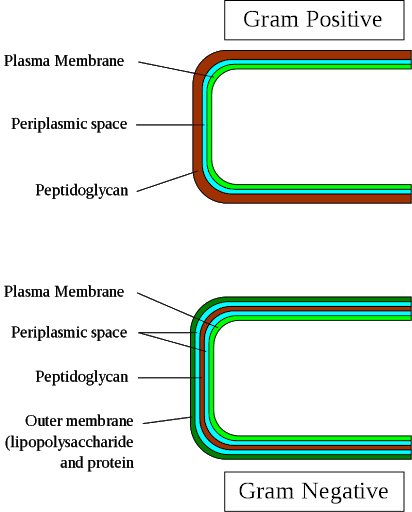
\includegraphics[scale=0.3]{Kap2/grampos1.png}
    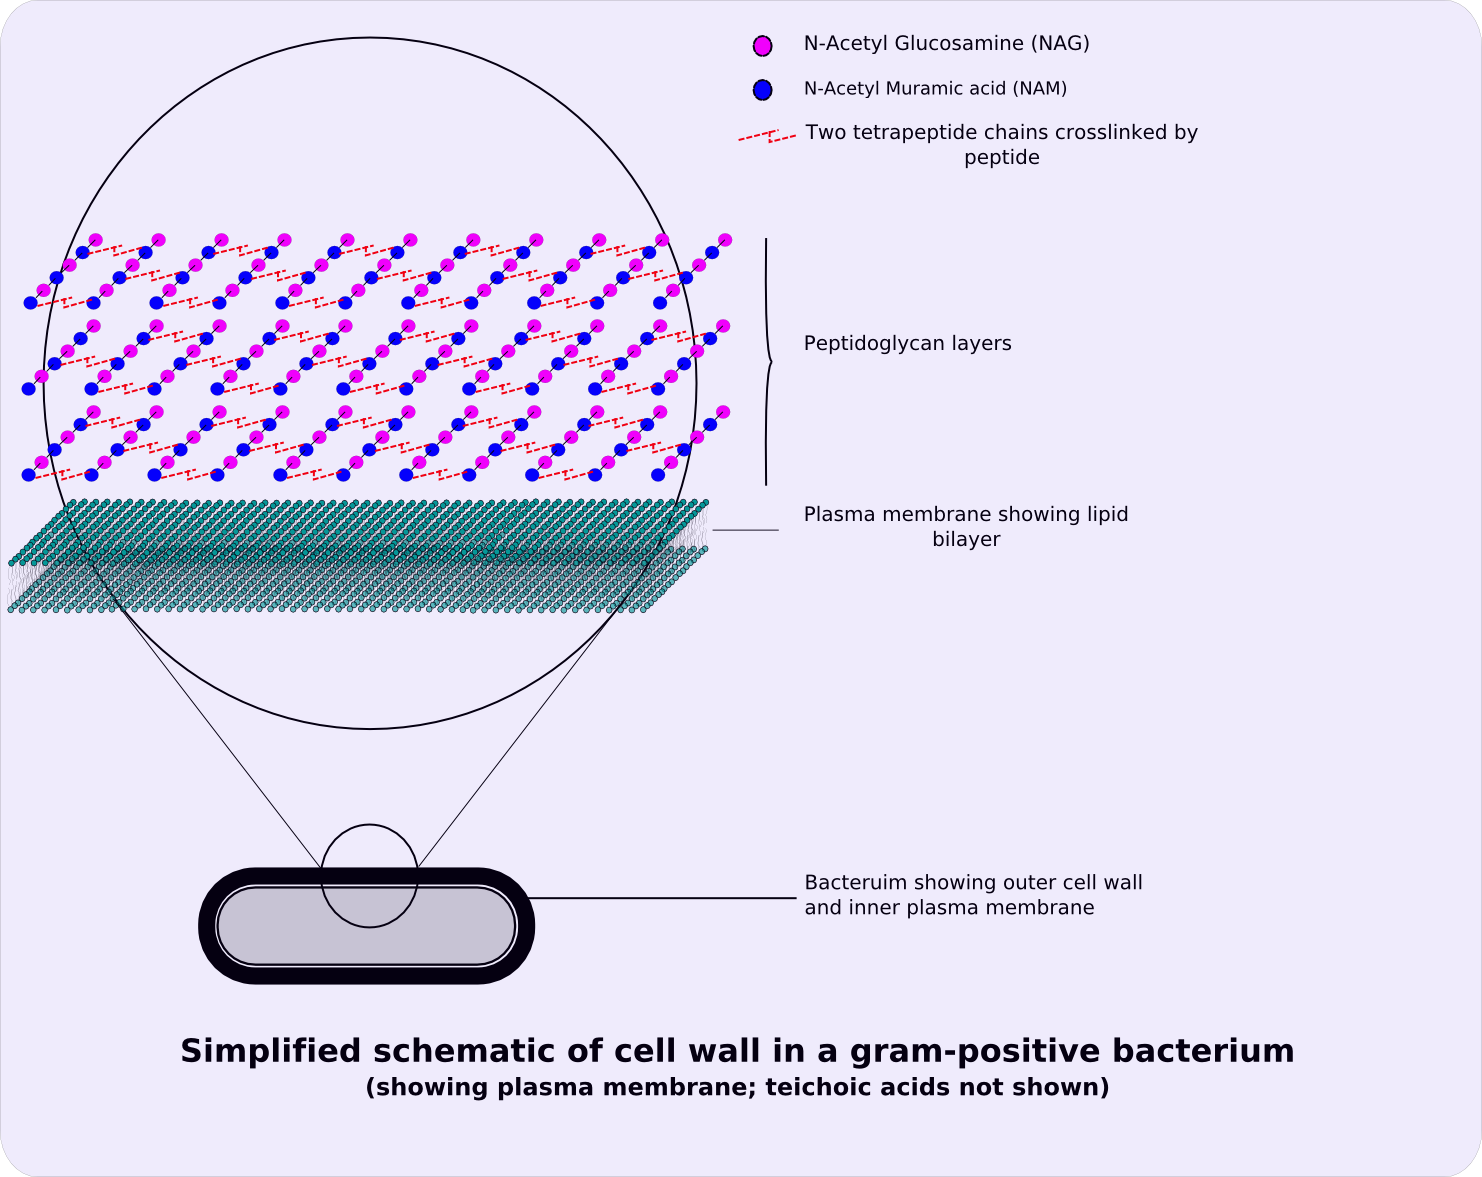
\includegraphics[scale=0.15]{Kap2/grampos2.png}
  \caption{Imagen  de la membrana de una bacteria Gram positiva. Tomado de \cite{Nelson2011}.}
  \label{fig:mem}
\end{center}
\end{figure}
La bicapa lip\'{i}dica es una membrana presente en todos las c\'{e}lulas la cual est\'{a} compuesta mayoritariamente por l\'{i}pidos. Los l\'{i}pidos se acomodan de tal manera que el espesor de la membrana sea de dos l\'{i}pidos de grosor. En su mayor\'{i}a, con excepciones como los esteroles, los l\'{i}pidos est\'{a}n compuestos por una o varias cadenas de \'{a}cidos grasos no polares (cadenas hidrocarbonadas con carboxilo) unidas a diferentes sustituyentes polares los cuales pueden presentar carga o no a pH fisiol\'{o}gico. De acuerdo a los sustituyentes y al tipo de \'{a}cidos grasos, cada l\'{i}pido presenta propiedades fisicoqu\'{i}micas espec\'{i}ficas como la carga total, la polaridad, y el largo que lo distinguen a nivel biof\'{i}sico con los otros l\'{i}pidos. Los l\'{i}pidos forman bicapas debido a la presencia del agua ya que al ser mol\'{e}culas anfip\'{a}ticas (combinando motivos polares y apolares) se orientan con respecto a esta. La parte hidrof\'{i}lica del l\'{i}pido interact\'{u}a con el agua mientras que la parte hidrof\'{o}bica no interact\'{u}a con esta, lo que induce reorientaci\'{o}n y agregaci\'{o}n de los l\'{i}pidos. Estas interacciones hacen que sea m\'{a}s estable encontrar los l\'{i}pidos inmersos en el agua formando agregados sin mezclarse con el agua. La interacci\'on lateral entre estas mol\'eculas se da a trav\'es de fuerzas no covalentes lo que le confiere propiedades de cristal l\'iquido caracterizado por la capacidad de presentar transiciones de fase s\'olido-l\'iquido y difusi\'{o}n lateral. \\

La bicapa lip\'{i}dica de \textit{Staphylococcus aureus} esta compuesta principalmente por fosfatidilgliceroles (PG), cardiolipina (CL), lifosfoglicandos (LPG) y glicopeptidol\'{i}pidos (GPL) \cite{Sohlenkamp2015BacterialPathways}. En la figura \ref{fig:DMPG} se muestra la f\'{o}rmula estructural del Dimiristoilfosphatidilglicerol (DMPG), el cual es un l\'{i}pido con el fosfatidilglicerol unido a dos miristoil (provenientes del \'{a}cido mir\'{i}stico). 
\\

\begin{figure}[h]
\begin{center}
    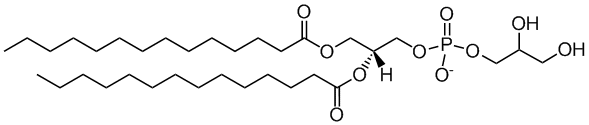
\includegraphics[scale=0.4]{Kap2/DMPG.png}
  \caption{F\'{o}rmula estructural del Dimiristoilfosphatidilglicerol (DMPG). Tomada de \cite{CHEMDRUGDMPGDimyristoylphosphatidylglycerol}.}
  \label{fig:DMPG}
\end{center}
\end{figure}
Las membranas lip\'{i}dicas adem\'{a}s de tener l\'{i}pidos contienen otros tipos de biomol\'{e}culas como los carotenoides, las prote\'{i}nas y los glicol\'{i}pidos que tienen relevancia fisiol\'{o}gica en la c\'{e}lula. Los carotenoides en particular pigmentan las c\'{e}lulas. En el caso de \textit{Staphylococcus aureus} se ha descubierto que los carotenoides juegan un papel importante en la integridad de la membrana celular y protegen a la bacteria frente a estr\'{e}s oxidativo \cite{Nagendra2011}. La protecci\'{o}n de los carotenoides en la membrana se ve reflejada por un aumento de su rigidez, de forma similar al papel que juega el colesterol en la membrana eucari\'{o}tica. \\

Uno de los carotenoides m\'{a}s relevantes en \textit{Staphylococcus aureus} es la estafiloxantina la cual le da el nombre a la bacteria ya que le da un color a\'{u}reo. La estafiloxantina es un  triterpeno carotenoide que posee dos cadenas hidrocarbonadas. Una de ellas es un \'{a}cido graso parecido a otros acidos grasos de la membrana, caracterizado por ser saturado y con presencia de ramificaciones metiles. El otro es un \'{a}cido graso diaponeurosporenoico, que presenta insaturaciones conjugadas tipo trans y ramificaciones.  Las dos cadenas est\'{a}n unidas a un mol\'{e}cula de glucosa mediante enlaces tipo \'{e}ster, ver figura \ref{fig:stx}. Debido a los enlaces dobles conjugados de la cadena diaponeurosporenoica, esta es r\'{i}gida, ya que estos enlaces dificultan rotaciones intramoleculares. Esta rigidez se convierte en un factor que aumenta el empaquetado de la bicapa l\'{i}p\'{i}dica, ya que disminuye la distancia entre l\'{i}pidos vecinos \cite{Heimburg}.\\

\begin{figure}[h]
\begin{center}
  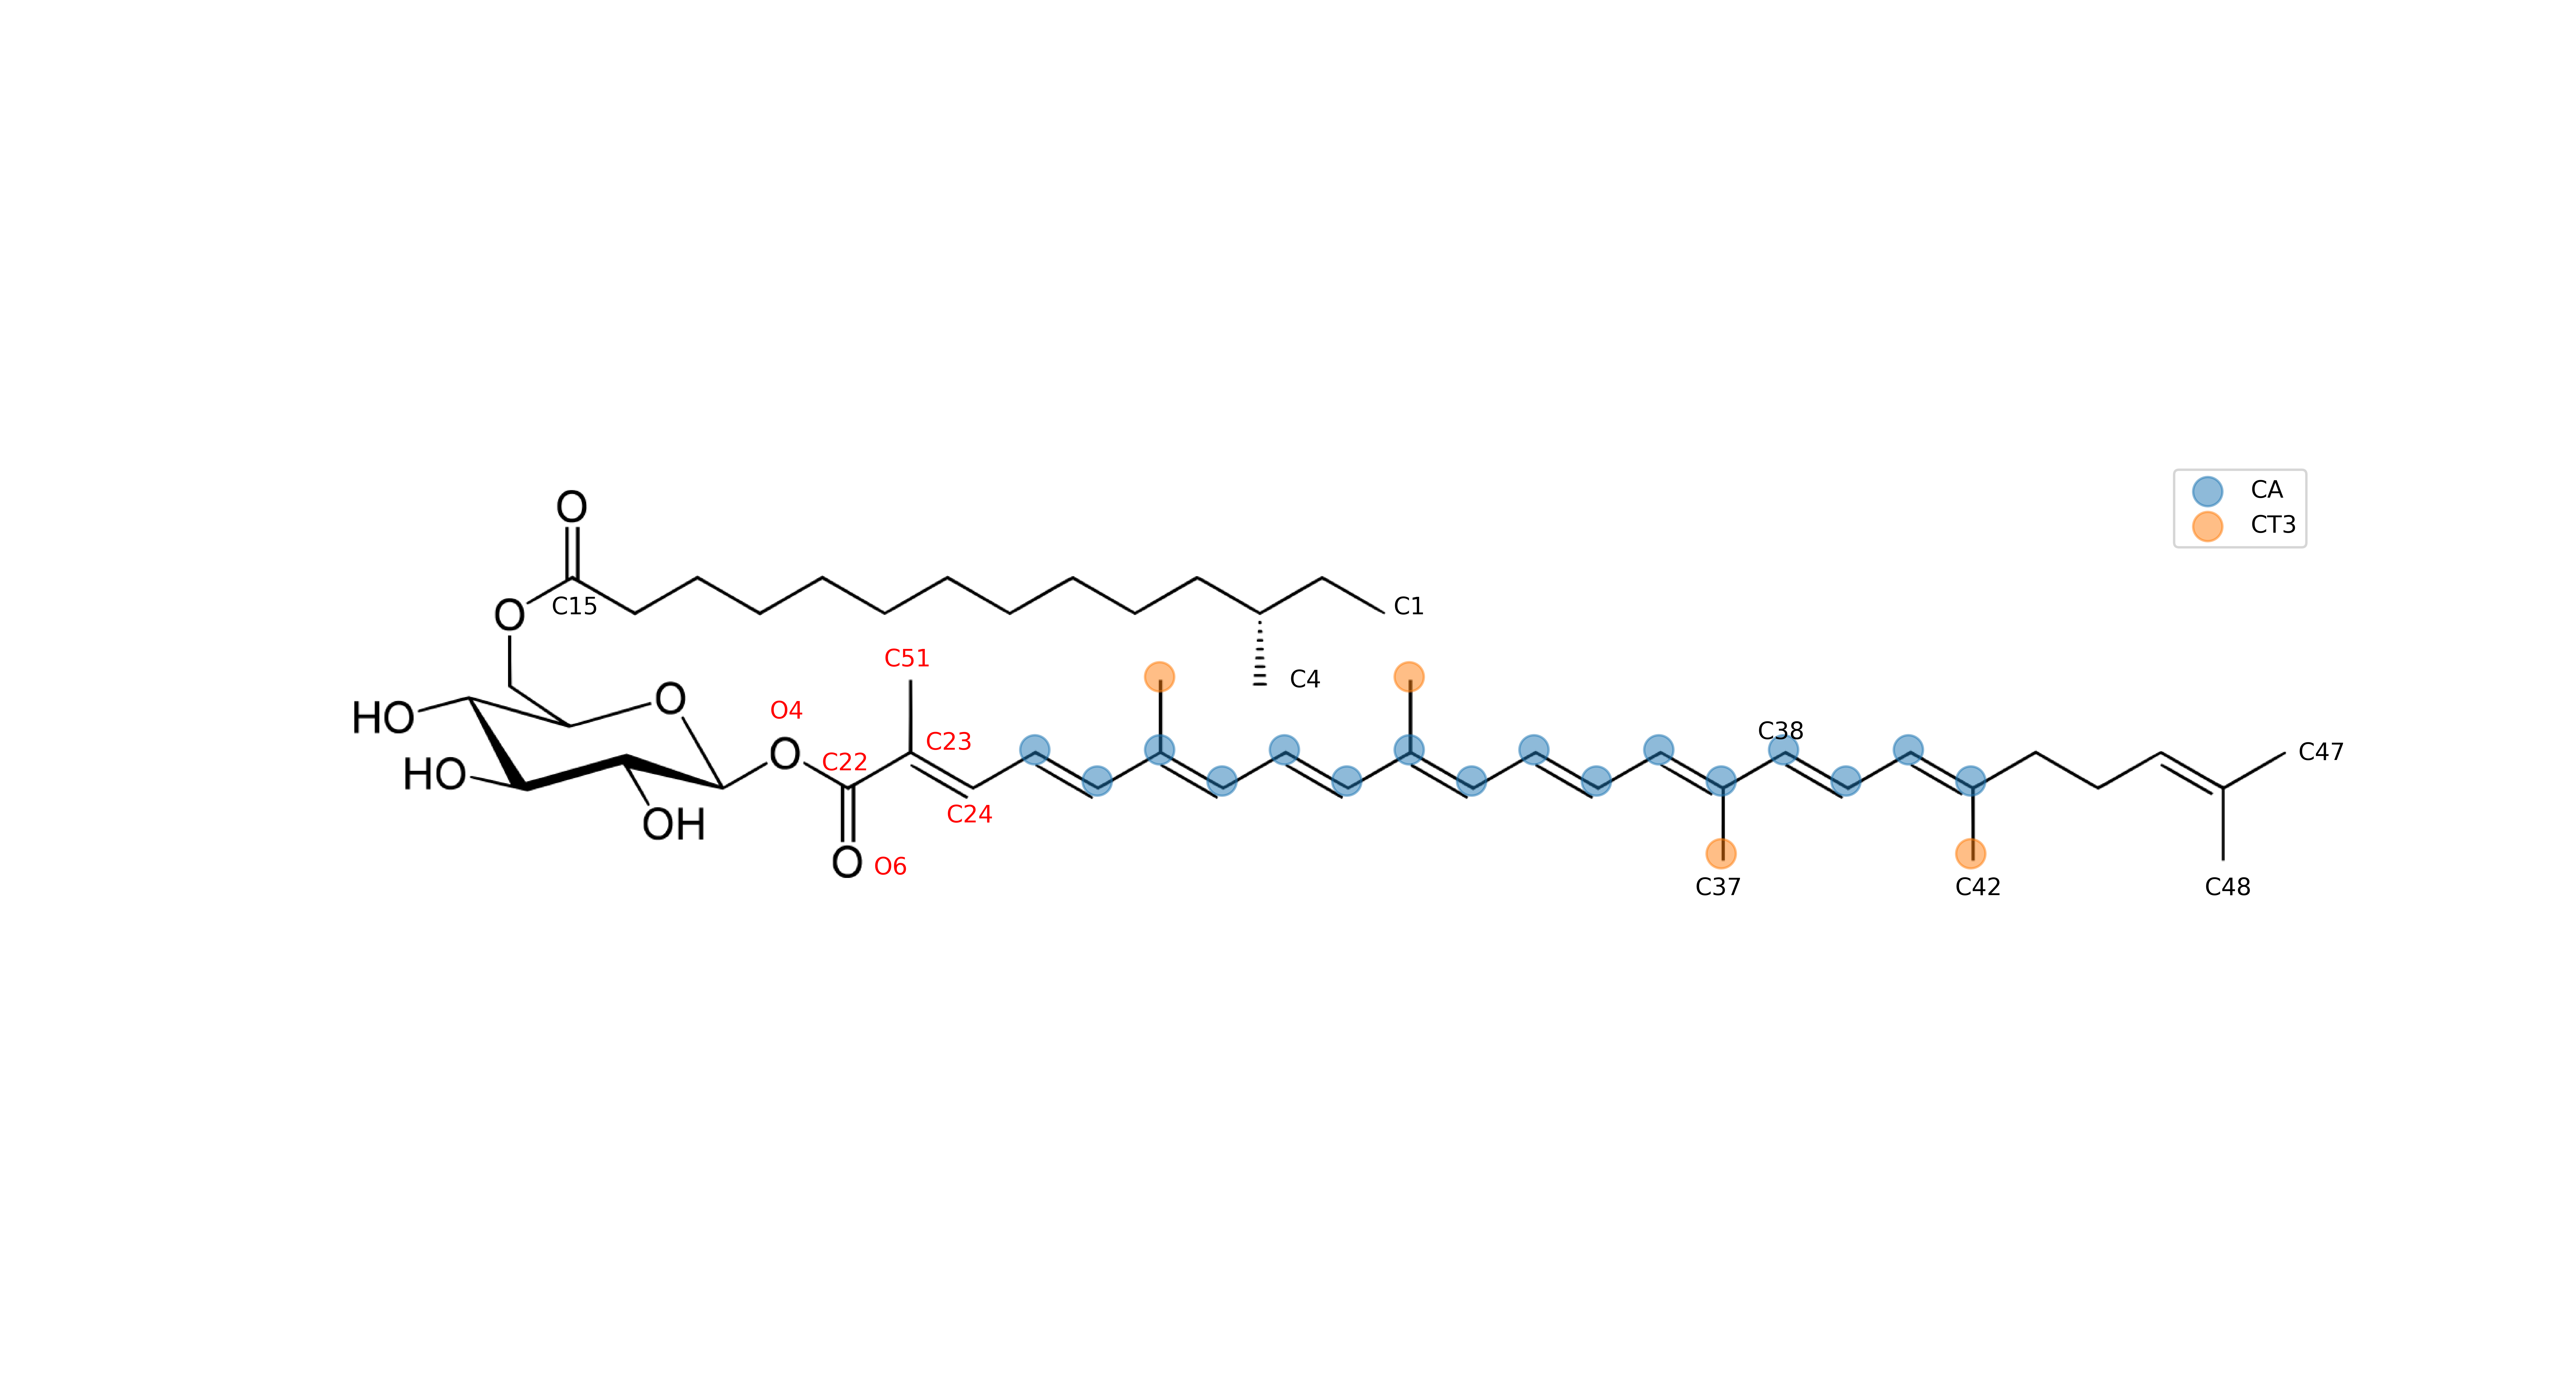
\includegraphics[scale=0.4]{Kap2/stx_problems.png}
  \caption{F\'{o}rmula estructural de la estafiloxantina. Tomada de \cite{MelendezDelgado2018StudyingBilayers}.}
  \label{fig:stx}
\end{center}
\end{figure}
 Adem\'{a}s, estas insaturaciones conjugadas le dan propiedades antioxidantes que protegen a la bacteria frente al estr\'{e}s oxidativo del medio, al poder incorporar especies reactivas oxidativas \cite{Nelson2011}.
\section{Resistencia a tratamientos antibi\'{o}ticos de \textit{Staphylococcus aureus}}\label{ss:anti}
Desde el descubrimiento de la penicilina, infecciones de \textit{Staphylococcus aureus} han sido tratadas con este antibi\'{o}tico. Sin embargo, a mediados del siglo XX \textit{Staphylococcus aureus} comenz\'{o} a presentar resistencia a esta familia de antibi\'{o}ticos $\beta$-lact\'{a}micos, incluida la meticilina. Posteriormente se han aplicado otros antibi\'{o}ticos como la vancomicina, pero tambi\'{e}n se ha ido generando  resistencia a estos otros antibi\'{o}ticos.  De la resistencia a antibi\'{o}ticos surge la necesidad de buscar nuevos medicamentos que combatan \textit{S. aureus}.\\

Un p\'eptido antimicrobiano es  un olig\'omero de amino\'acidos, de alrededor de 20 aminoacidos de largo, que hace parte de la respuesta inmune de un amplio espectro de especies, y que son faciles de sintetizar en el laboratorio. Los p\'{e}ptidos antimicrobianos se clasifican seg\'{u}n la estructura secundaria que tienen: $\alpha$ h\'elices, $\beta$ plegados.   Los p\'eptidos antimicrobianos interact\'uan con la membrana de la bacteria produciendo orificios que causan p\'erdida de contenido, p\'{e}rdida del potencial electroqu\'{i}mico y muerte celular.\\

Los p\'{e}ptidos antimicrobiales forman estructuras anfip\'{a}ticas que inducen su adhesi\'{o}n a la membrana. Al aumentar su concentraci\'{o}n superficial, se induce una inserci\'{o}n de estos p\'{e}ptidos, atravesando la membrana y generando poros. Son de inter\'{e}s los p\'{e}ptidos antimicrobiales cati\'{o}nicos ya que la membrana de \textit{Staphylococcus aureus} es ani\'{o}nica y estos p\'{e}ptidos tienen una preferencia para adherirse a estas membranas. La formaci\'{o}n de poros es un proceso mec\'{a}nico que requiere la deformaci\'{o}n de la membrana para suceder. Al incrementar la rigidez de la membrana, se dificulta la inserci\'{o}n del p\'{e}ptido generando resitencia \cite{Perez-LopezVariationsProperties}, \cite{Nagendra2011}. Por este motivo se vuelve relevante estudiar como la composici\'{o}n de la membrana, en particular la presencia de stafiloxantina, modula la rigidez de la membrana.
